For the final Milestone, each group member was required to individually implement different Barrelfish subsystems and then jointly integrate them at the end. This chapter delves into \textit{networking} and was completed by \textbf{Adrian}.
\\\\
Due to time constraints I was not able to get this milestone done, so the majority of this chapter is written from a ``what if" perspective. All design here is theoretical and may gloss over some finer details that only would have been revealed during the implementation process.

\subsection{Introduction}
A modern OS is not very useful without some way to communicate with the outside world. In order to achieve this, they all implement what is known as a \textit{networking stack}, which is responsible for carrying out all of the necessary functionality in order to achieve network connectivity for the host machine.
\\\\
In this section, I describe the design and (theoretical) implementation of a simple networking stack for our OS. For this project in particular, I was to implement the ARP protocol, the ICMP protocol, a simple UDP echo server, and the ability to run multiple echo servers in separate processes.

\subsection{Virtio-net Driver}
In order to implement any of the aforementioned protocols, the system must be capable of sending and receiving raw network packets in the first place. This was achieved by writing a basic driver, which was layered on top of the provided virtio-net driver. The virtio-net driver is a specific implementation of the \textit{Virtio} device interface, which abstracts away the underlying register interface and hardware descriptor queues of the (virtual) Network Interface Card (NIC) used within QEMU. In general, such a device utilizes memory-mapped I/O (MMIO), which is where the device's registers are accessed by certain regions of computer memory mapped to them.

\subsubsection{Device Queues}
In order to pass data between the driver and the device, the virtio-net interface defines abstract \textit{send} and \textit{receive} queues that we can use. Under the hood, these queues refer to hardware descriptor queues of the NIC, which store information about each packet that is stored within memory, such as its address, size, etc. The driver defines a region of memory and then splits it into distinct \textit{buffers}. These buffers can be either "owned" by the driver or by the device. If a buffer is driver-owned, the driver can read from or write to them. If a buffer is device-owned, the device can read from or write to them - if the driver attempts to do so, the behaviour is undefined or results in an error. Buffers are enqueued to the device and dequeued from the device back to the driver to facilitate exchange of data between the two.

\subsubsection{Sending and Receiving Packets}
In the driver, sending a packet requires a few steps:
\begin{itemize}
    \item copy data from the packet into a driver-owned transmit (tx) buffer
    \item enqueue the tx buffer to transfer ownership to the device (the device will send the data)
    \item dequeue the tx buffer once the data has been sent (the device no longer needs it, the driver can reclaim it to use it further sends)
\end{itemize}
Similarly, to receive a packet, the following steps must be taken:
\begin{itemize}
    \item enqueue a receive (rx) buffer to transfer ownership to the device (the device will write a received packet into it)
    \item dequeue the rx buffer once the data has been written into it by the device
    \item retrieve the data from the rx buffer
\end{itemize}
There is some design freedom with when the relevant buffers are enqueued and dequeued. The rx buffers don't need to stay in the driver and can remain in the device queue to be ready to receive incoming packets at any time, and similarly the tx buffers don't need to stay in the device queue as the driver may want to send a packet at any time. To gain some performance, these operations should ideally be done when the associated sending/receiving is not being performed and the device is essentially "idle". Otherwise, the driver spends time transferring buffers when they should already be ready for it to use.
\\\\
There is also a choice to be made of whether or not sending and receiving are to be performed in a blocking or non-blocking fashion. Blocking send/receive calls have the benefit of simplicity in terms of programming, but they generally incur a significant hit to performance, as the process servicing the request could be running another thread while the driver thread waits on the device. On the contrary, non-blocking calls, while more performant, are more difficult to use as a programmer. Also, non-blocking calls do not benefit much from performance increases if the underlying operation does not take an exceedingly long time and is happening frequently enough, as context switches have a non-negligible cost in CPU cycles. Depending on the use-case, either option may be better-suited over the other.

\subsection{Network Stack}
While not explicitly stated in the project instructions of this milestone, it is clear that some sort of networking stack is intended to be designed. A networking stack is simply the collective design and implementation of a set of network protocols the system is meant to handle. It is a layer that is considered above any network driver that is being used by the system, and is responsible for all processing and handling of incoming and outgoing packets. This entails things such as:
\begin{itemize}
    \item \textbf{Determining the type of packet}: for both incoming and outgoing packets, the network stack would be called upon (by the driver in the former case, by the network-stack-invoking application in the latter) to determine what type of packet it is meant to deal with.
    \item \textbf{Encoding/decoding packets}: once the network stack knows what type of packet it is dealing with, it must then correctly encode or decode it by adhering to whatever protocol it has detected.
    \item \textbf{Sending the resulting data to the appropriate layer}: if the network stack was called upon to send data, the encoded packet now must be passed onto the driver for it to be sent from a network interface. In the case that it has received and decoded a packet, the decoded data now must be passed onto the application which it is destined for, determined usually by the port contained within the transport layer of the packet.
\end{itemize}

\subsubsection{Possible Designs}
In general, the network stack must expose some sort of API for the protocols it has implemented that applications can call upon to carry out the desired networking functionalities. The application interface would contain functions that call upon the network stack to carry out a particular protocol with the data passed in. Conversely, the driver interface would be relatively simple and contain fewer functions that generally only need to call upon the network stack with the data that was just received by the driver. The network stack would be responsible for figuring out what protocol the packet is using, and passing it onto its appropriate processing functions. Of course, it is entirely possible there is more design to be had with the network stack itself that I am unfortunately not able to realize as I had not had the chance to implement this yet by the time of writing.

\subsection{ARP Protocol}
A common case that arises in networking is when a machine \textbf{A} (more accurately, a network interface) knows the IP address of another machine \textbf{B} in its local network. One way in which this can happen is by way of a local DNS exchange, for example. In order for \textbf{A} to send data to \textbf{B} over the link that connects them, \textbf{A} must know \textbf{B}'s \textit{MAC address}. To enable the discovery of this address with a known IP address, the ARP protocol can be used. In terms of network layering, ARP is atypical as it doesn't clearly fall within one layer - in general, it can be said to be simultaneously a link-layer and network-layer protocol, due to the fact that it necessarily uses information from both.
\\\\
In this milestone, a simplified ARP protocol was implemented that is capable of achieving MAC address discovery and caching. The protocol uses a special ARP packet, which contains the ARP header, and is encapsulated by a link-layer Ethernet header. The packet is relatively simple (see figure \ref{figure:arp-packet}) - three fields are of particular importance: 1) the destination IP (machine \textbf{B}), 2) the source MAC address (machine \textbf{A}), and 3) the destination MAC address.
\begin{figure}[ht]
    \centering
    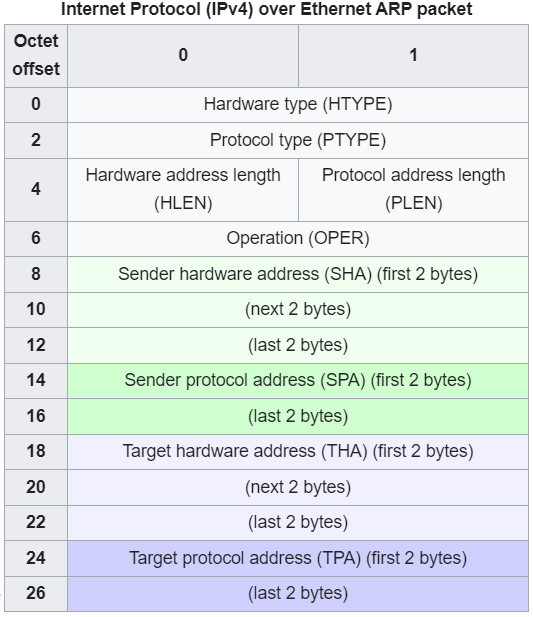
\includegraphics[width=0.6\columnwidth]{images/m7-networking-arppacket.png}
    \caption{Layout of an ARP packet. \cite{wikipedia}}
    \label{figure:arp-packet}
\end{figure}
A more complete ARP protocol implementation involves more functionalities such as probes, announcements, etc. For the purposes of this milestone, only MAC address discovery was implemented. This only requires two message types:
\begin{itemize}
    \item \textbf{ARP request}: machine \textbf{A} does not know machine \textbf{B}'s MAC address, so in its ARP packet it fills in a special \textit{broadcast} destination MAC address of FF:FF:FF:FF:FF:FF. All machines in the local network will receive this packet, and by the protocol only the machine with the destination IP address must respond with a reply.
    \item \textbf{ARP reply}: machine \textbf{B} sends back an ARP packet through the local network with the source and destination fields inverted, with the exception of what is now the source MAC address. Instead of the broadcast address, it fills in its MAC address to be sent back to the requesting machine.
\end{itemize}
Caching of ARP requests and replies was also implemented. This was relatively simple and involved the use of a hash table, as provided from the \textit{collections} library. If the machine received an ARP request, it would store the source IP $\rightarrow$ source MAC mapping within the cache, as well as sending back the reply. Upon receiving the reply from an initial ARP request, the same thing would be done with the destination IP and MAC address.

\subsection{ICMP Protocol}
The ICMP protocol is a network-layer protocol that is used to send error and other operational information between devices operating at that layer. In this milestone, however, we are only concerned with the implementation of sending ping packets.
\\\\
A ping packet is simply an ICMP packet where the "type" and "code" fields are both 0. When a machine that implements this protocol receives such a packet, it is simply to send back the same packet to its source. There are a few quirks with this protocol that would need to be handled, however, such as the $DF$ flag being set within the IPv4 header. This flag states that the overall packet being received is too large for the underlying network hardware to take in as a single packet, and it must be fragmented. Normally, a network stack would be responsible for re-assembling the packet, but this is not required for the purposes of this project. This ICMP protocol implementation is simply to drop such a packet.
\\\\
An important part of implementing the IP protocol is error-checking. This is implemented by a simple checksum algorithm which takes the one's complement sum of all the IP header words, then takes the one's complement of this resulting value. Upon reception of a packet containing an IP header, this checksum is checked against the entire header - if the value is not what is expected, the network stack is to interpret this as an error and drop the packet. For this project, a simple function was available to use to calculate the checksum.

\subsection{UDP Echo Server}
This part of the milestone involves setting up a simple echo server using UDP with a hard-coded port. There is not much design to be had here, as the implementation (had I carried it out) is rather prescriptive.
\\\\
With a working ping functionality from the previous part, a process would then be setup to be running in an infinite loop, which keeps attempting to receive packets. Upon reception, it would simply hand the packet off to the network stack to be processed, as was described previously. In the case of the echo server, a received ping packet would result in an identical packet being sent back to the source IP and port over UDP.

\subsection{Multiple Clients}
This part of the milestone involves setting up a generalized networking service which other processes within the OS can use. For our OS, the API would be an RPC interface. Each RPC call would call upon a particular function within the stack that would carry out a particular protocol, as discussed previously. However, the question is then this: how exactly is the underlying driver running that the network stack is passing its data down to?

\subsubsection{Possible Designs}
One possible way in which the driver could run is directly within the \textit{init} process. This is a design that we had used for milestone 4 and onwards, mostly because of its simplicity. This special process has certain capabilities already set up for us that makes starting a service within it much easier, and the same is true for the network driver - the device frame capability is directly exposed to the driver, and it can just use it. The existing RPC bindings to \textit{init} can also be used, and not much additional setup to expose this service would be required. However, there is the downside of performance with this approach, especially because of the fact that we already have multiple services (memory management, process management, etc.) that \textit{init} is running.
\\\\
On the contrary, the performance gains from running the driver in its own process is clear, as that process would only be responsible for serving RPC requests for networking functionalities. With this design, however, other processes must then know how to bind to this one in order to be able to make such calls in the first place. Our binding interface that was fleshed out to handle UMP as well as LMP in milestone 6 is capable of this, but only between a process and \textit{init}. We would need to be able to carry out arbitrary bindings between two processes, of which one way this could be achieved is with a working name server. The networking server would register itself with the name server, and other processes would be able to query this name server to get a binding to the networking server.

\subsection{Challenges}
This milestone was particularly challenging due to environment setup issues. With only minor modifications required to given build files associated with this project (that took me a long time to realize), there was still an issue with how I had been running QEMU. I had been using WSL2, which is essentially a Linux VM running within my host Windows 11 OS, and this VM is then running QEMU. With a lot of investigation, I came to the conclusion that it's not possible (or at least I won't figure it out in a reasonable amount of time) to send packets from the OS running within QEMU, which has to make it past whatever virtual network interface(s) there is/are at the QEMU - Linux boundary, and then past the Windows - WSL boundary. With a WireShark instance running inside WSL, I can see that packets successfully make their way outside of QEMU, but no such packets ever make it outside of WSL. As a result, the only way in which I was able to test my code was to send packets to a network interface within WSL itself, which had its own quirks in and of itself (such as a dynamically-changing MAC address).
\\\\
There is also a challenge unique to debugging networking implementations, and that is stray packets being received that you do not expect. At first, they appear to be packets that you intended to receive based on what was just sent, but one then may realize that other packets from mostly-unknown sources can be randomly sent at any time. In order to combat this, reception just has to run for long enough to make sure there was ample time for the expected packets to arrive, and to ignore other packets. Naturally, this lends itself to the strategy of simply dropping and packets the network stack does not know how to handle.